\documentclass[12pt]{report}
%================================================================
% Preamble declarations
%----------------------------------------------------------------
% For instructions regarding the Graduate Office style, see:
%   http://www.nmt.edu/tcc/help/pubs/nmtthesis/
% For instructions regarding the nmtthesis2013.sty package, see:
%   http://www.nmt.edu/tcc/help/pubs/nmtthesis/latex2013/
%----------------------------------------------------------------
% Place \usepackage commands for other modules here
\usepackage{natbib}% Example bibliographic style
%
% Use the NMT 2013 thesis style
%
\usepackage{nmtthesis2013}
\usepackage{pdfpages}


%
% Select the type of publication, one of these three.
%
\dissertation
%
% General options
%
\author{Jake Ross}
\title{Geochronology of Southern McMurdo Sound and development of a micro laser furnace}
\degree{Doctor of Philosophy}
%
% If you leave the following line commented, the date will be
% the next available month and year of graduation ceremonies
%
\graduationdate{April, 2014}

% Name your chairperson here.  Do not use titles such as Dr. or Ph.D.
%
\chair{William C. McIntosh}
%
% Number of people on your committee include chair(s)
%
\committeesize{5}
%================================================================
\begin{document}
%
% Begin front matter
%
%----------------------------------------------------------------
\begin{dedication}
{To my arrow...}
\end{dedication}
%----------------------------------------------------------------
%
% Produce the title page
%
\titlepage
%----------------------------------------------------------------
%%%%\epigraph[who said it]{what they said}
%----------------------------------------------------------------
%%%%\frontispiece[title of the graphic]{some graphic}
%----------------------------------------------------------------
%
% An abstract is required.  For suggestions on its content, see:
%   http://www.aapg.org/bulletin/abstract_scrutiny.pdf
% After your abstract, provide two to six keywords, or key 
% phrases of up to three words, to assist librarians in
% indexing your work.
%
\begin{abstract}
Minna Bluff has been a significant topographic barrier to the flow of the Ross Ice Shelf since the mid-Miocene. Detailed Ar-Ar analyses of kaersutite and sanidine phenocrysts, and groundmass concentrates from volcanic units indicate an overall west to east progression of volcanic activity.  Eruptions of basaltic to intermediate lavas, domes, and scoria cones started at ~12 Ma in at what is now the eastern most point of Minna Bluff, “Minna Hook.” Activity was centered in this area for ~4 Ma, constructing a pre-Minna Bluff island. Multiple glacial unconformities found at Minna Hook suggest repeated interaction with large warm-based, erosive ice sheets. Activity migrated westward from Minna Bluff Island at 7-8 Ma closing the gap created by the island and the mainland. Significant edifice construction continued until 4-5 Ma with sporadic and parasitic scoria cone eruptions, possibly associated with Mt. Discovery activity, continuing until 2 Ma. 

The orientations of Minna Bluff’s two major axes are strongly controlled by regional tectonic features. Minna Bluff’s E-W axis, McIntosh Cliffs, is sub-parallel to the Radial Lineament and the N-S axis, Minna Hook, appears as extension of faulting bounding the Terror Rift. The constructional evolution of the 70km long volcanic complex has an important role in interpreting the climate signals recovered by the ANDRILL Project. Minna Bluff influenced the material delivered to the AND-1B drill site (ANDRILL MIS 2006-2007) in three critical ways: 1) Minna Bluff diverted upstream material, 2) provided

a pinning and stabilizing point for the Ross Ice Shelf, possible controlling the calving line prior to the emergence of Ross Island, and 3) was a significant source of fresh volcanic material throughout much of the period recovered by ANDRILL MIS. For example, a kaersutite-bearing clast recovered from 822.78 mbsf in AND-1B yielded an age of 8.53±0.51 Ma, and was likely derived from Minna Bluff.  The results from this study can be incorporated into detailed glacier and ice-sheet models of the McMurdo Sound region, a critical area in the Ross Ice Sheet and global climate system. \cite{Jourdan:2007vi}

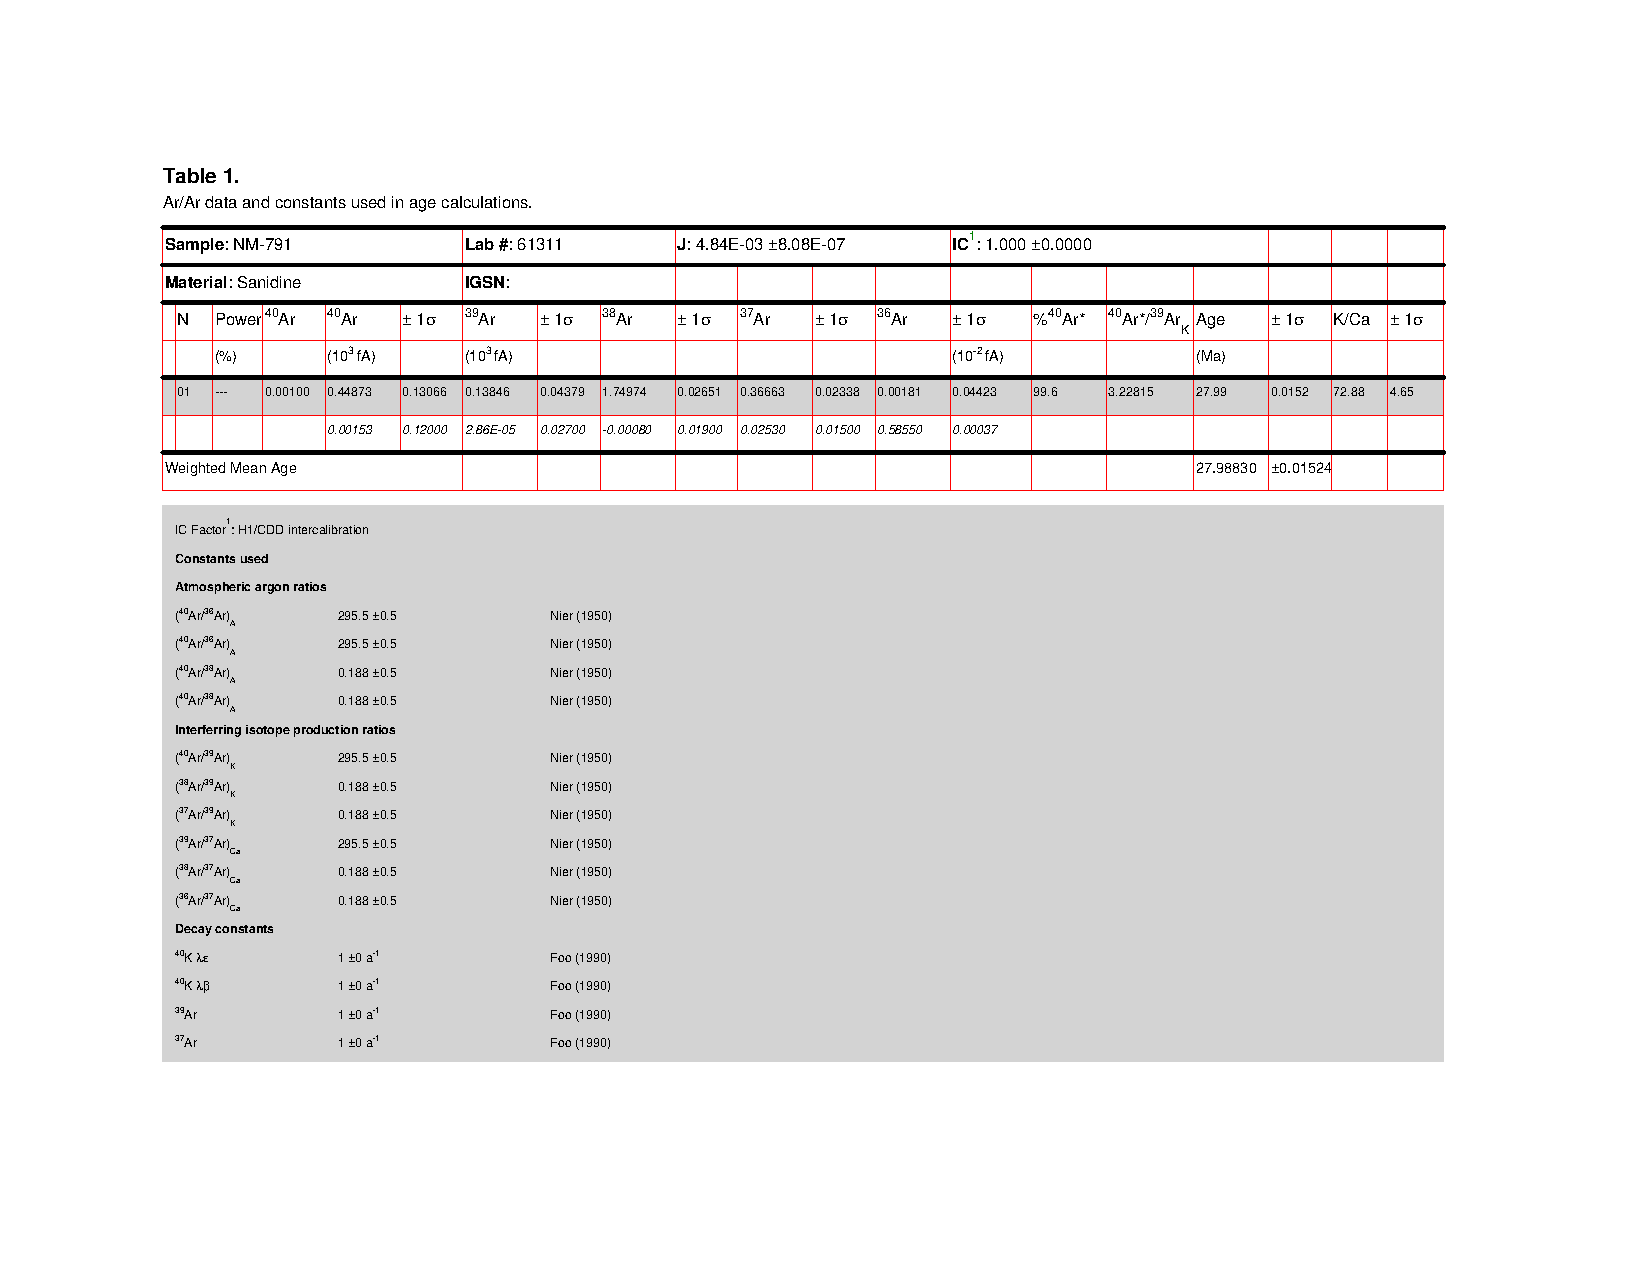
\includepdf[pages={-}, landscape=true, addtolist={1, table, Table 1., foo1}]{table.pdf}

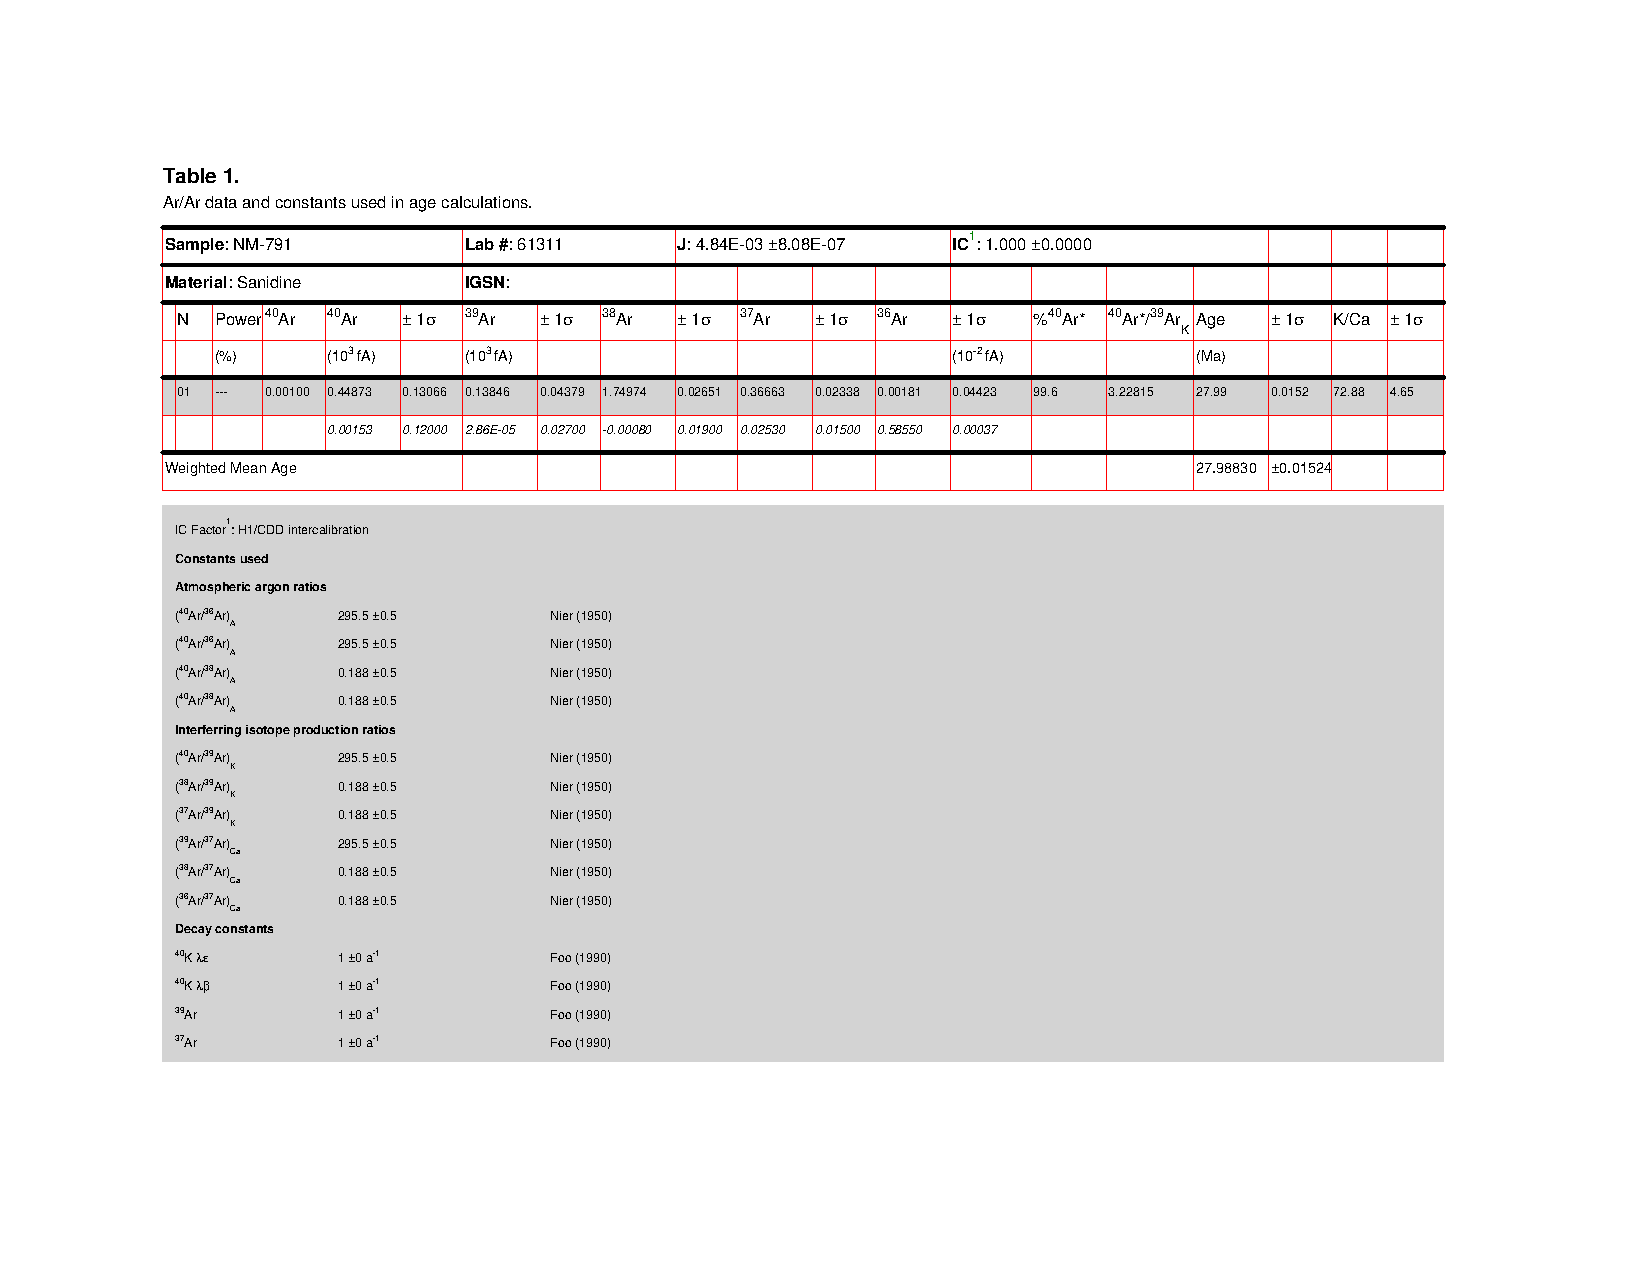
\includepdf[pages={-}, landscape=true, addtolist={1, table, Table 2., foo2}]{table.pdf}

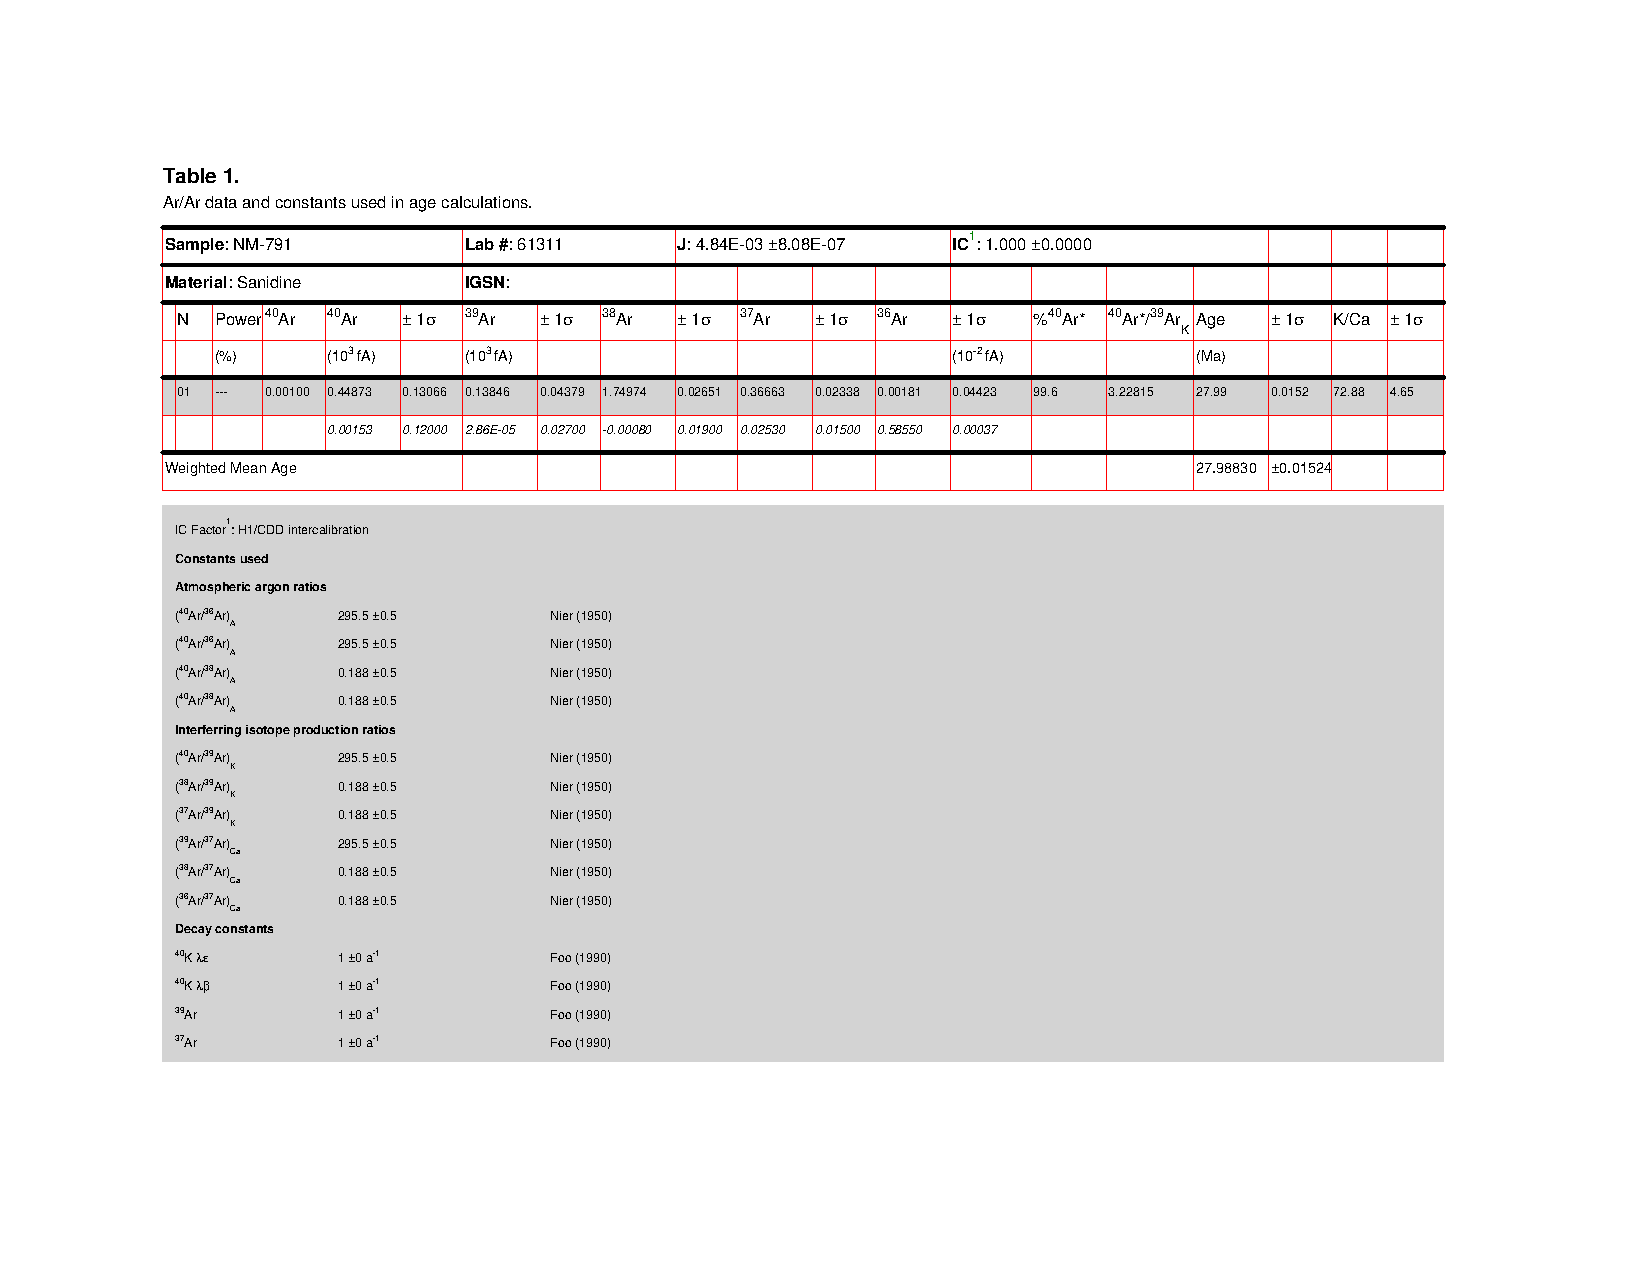
\includepdf[pages={-}, landscape=true, addtolist={1, table, Table 3., foo3}]{table.pdf}

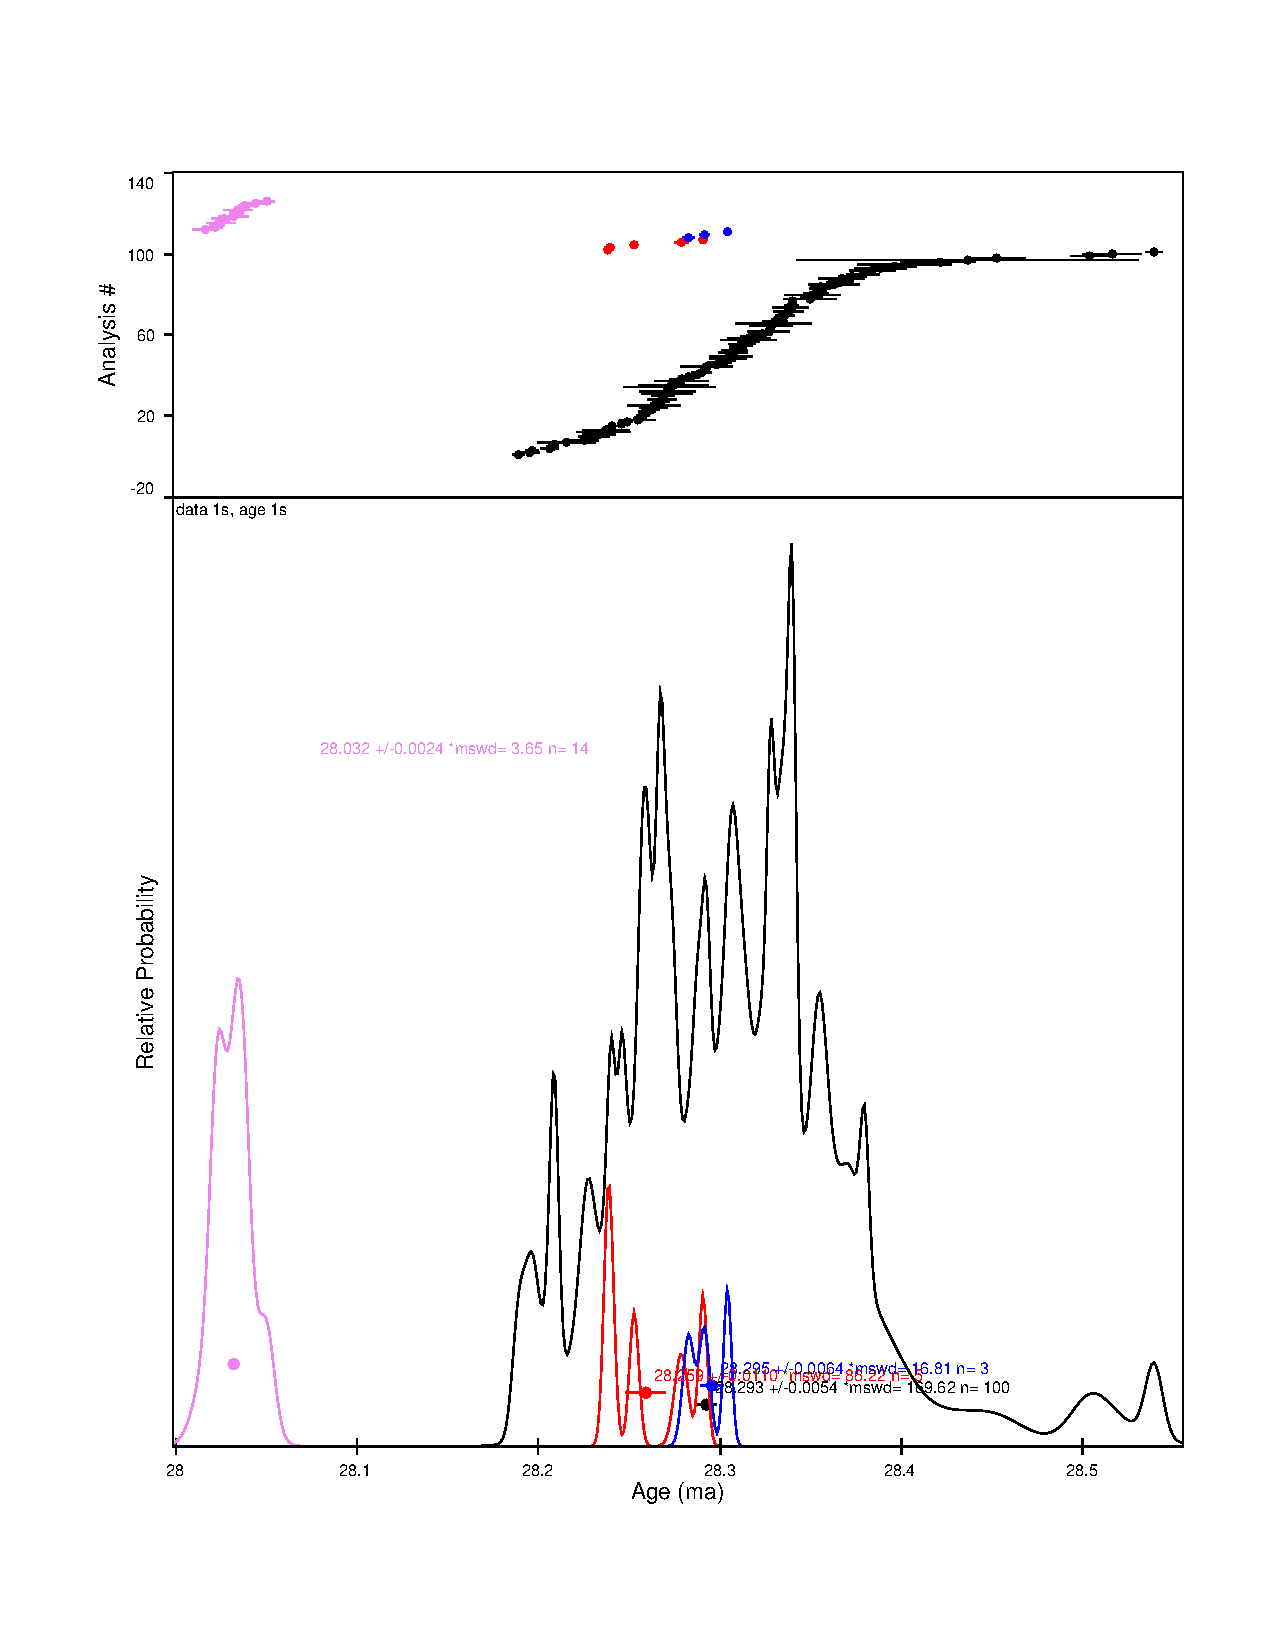
\includepdf[pages={-}, landscape=true, addtolist={1, figure, Figure 1., foo3}]{figure.pdf}





\keywords{A; B; C}
\end{abstract}
%----------------------------------------------------------------
\begin{acknowledgments}
{Foo}

\end{acknowledgments}
%----------------------------------------------------------------
\tableofcontents
%
% If you have no tables, comment out \listoftables.
% If you have no figures, comment out \listoffigures.
% If you provide a List of Abbreviations, create a file
%   'abbrs.tex' containing the abbreviations table, and
%   uncomment \listofabbrs.
%
\listoftables
\listoffigures
%%%%\listofabbrs
%----------------------------------------------------------------
\signaturepage
%----------------------------------------------------------------
\begin{preface}
{Foo}
\end{preface}
%================================================================

\chapter{Development of an age-depth model for ANDRILL MIS AND-1B drill core, McMurdo Sound, Antarctica}
\chapter{Geochronology of Minna Bluff, Southern McMurdo Sound, Antartica}
\section{Introduction}
Minna Bluff is a large volcanic penisula 70km south of Ross Island, Antarctica
\section{Geology}
\subsection{Volcanic}
This section describes the glacial geology of Minna Bluff. Here is the text
wrapping around and a displaying a the outer indentation
\subsection{Glacial}
This section describes the volcanic geology of Minna Bluff. Here is the text
wrapping around and a displaying a the outer indentation
\section{Methods}
\subsection{Ar-Ar}
\section{Results}
\subsection{Ar-Ar Laser Fusion}
\subsection{Ar-Ar Step Heating}
\section{Discussion}
\chapter{Development and Testing of a laser micro furnace for Ar-Ar analysis}
\section{Design}
\section{Testing}
\section{Preliminary Results}
\chapter{Pychron: Noble gas data acquisition and processing framework}

\appendix
\chapter{Ar-Ar data}
\chapter{Electron Microprobe data}



\nocite{*} %% adds all references in bib files to ref list

%================================================================
% References section.  Uncomment one of the next two commands,
% depending on whether you cite references by number, or by
% author and year.
% 
% For numbered citations:
%
%%%%\begin{References}[99]
%
% For citations by author and year:
%
\begin{References}[99]
%
% Inside the References environment, use these lines if you are
% using BibTeX.  Replace 'apalike' with the name of your style
% if you are not using APA-like citations.  Replace FILE1, FILE2,
% with the name(s) of your BibTeX database(s).
%
\bibliographystyle{apalike}
\bibliography{andrill,minna_bluff,diode,pychron}
\end{References}
\copyrightpage
\end{document}
